\documentclass{homework}
% \usepackage{graphicx} % Required for inserting images
\usepackage{amsmath}
\usepackage{gensymb}
\usepackage{subfig}
\usepackage{float}
\usepackage{pythonhighlight}

\class{APPM 5600}
\title{Homework 2}
\author{Sean Jennings}
\date{September 12, 2024}

\begin{document}
\maketitle

\section{Problem 1}
The bisection code is embedded at the end of this document.
\begin{letterenum}
\item The bisection algorithm found a root of 4.999965820312501 for $(x-5)^9$. This is within the given tolerance
of the known solution of 5.
\item The algorithm returns a root of 5.12186279296875 for the expanded polynomial.
\item When finding the root based on the binomial expansion of the function, floating point error is introduced. Let $a_k$
be the $k$th term in the binomial expansion, evaluated at $x=5$, given by:
\begin{equation*}
    a_k = {9\choose k} x^k (-5)^{n-k}
\end{equation*}

A numerical evaluation reveals that there are $k$ for which the absolute value $|a_k|$ exceeds 1e8. Since floating point
operations maintain a relative precision of about $1e-16$ the absolute error will be greater than 1e-8. 
For $x \in (4.9, 5.1)$, we have $|x - 5| < 0.1$ and thus $|x - 5|^9 < 1e-9$. Therefore,
the error is of greater magnitude than the function in some interval containing $[4.9,5.1]$.
The error causes the function output to change sign, causing the bisection algorithm to return the
erroneous root.

Figure (\ref{fig:f1-vs-f2}) illustrates the issue.


\begin{center}
    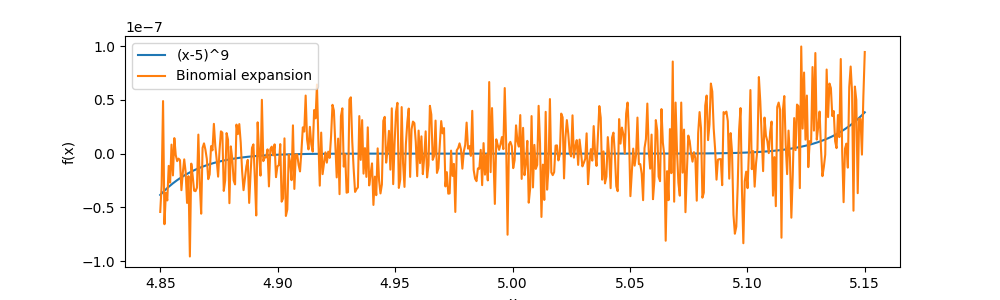
\includegraphics[width=\linewidth]{Images/f1_vs_f2.png}
    \captionof{figure}{Floating Point Error Introduced in Binomial Expansion}
    \label{fig:f1-vs-f2}
\end{center}
\end{letterenum}

\section{Appendix: Code}

\begin{python}
import math
import numpy as np
import matplotlib.pyplot as plt

EXIT_SUCCESS = 0
EXIT_FAILURE = 1


class BisectionResult:
    def __init__(self, root, exit_status):
        self.root = root
        self.exit_status = exit_status


def bisection(f, a, b, atol):
    fa = f(a)
    fb = f(b)
    if fa * fb > 0:
        return BisectionResult(
            a, EXIT_FAILURE
        )

    while abs(a - b) > atol:
        c = 1/2 * (a + b)
        fc = f(c)
        if fa * fc < 0:
            b = c
        else:
            a = c
            fa = fc
    return BisectionResult(
        a, EXIT_SUCCESS
    )


def f1(x):
    return (x - 5)**9

N = 9
COEFFICIENTS = [math.comb(N, k) * (-5)**(N-k) for k in range(0, N+1)]

def f2(x):
    return sum([coef * x ** k for k, coef in enumerate(COEFFICIENTS)])


def main():
    a = 4.8
    b = 5.31
    tol = 1e-4
    res = bisection(f1, a, b, tol)
    print("Bisection return status for (x-5)^9:", res.exit_status)
    print("Bisection root for (x-5)^9:", res.root)
    res = bisection(f2, a, b, tol)
    print("Bisection return status for expansion:", res.exit_status)
    print("Bisection root for expansion:", res.root)

    # Plot the functions in a region around the root.
    x = np.linspace(4.85, 5.15, 500)
    y_f1 = [f1(v) for v in x]
    y_f2 = [f2(v) for v in x]
    fig = plt.figure(figsize=(10,3))
    plt.plot(x, y_f1, label="(x-5)^9")
    plt.plot(x, y_f2, label="Binomial expansion")
    plt.legend()
    plt.xlabel("x")
    plt.ylabel("f(x)")
    fig.savefig("tex/hw2/Images/f1_vs_f2.png")
    plt.show()
    print("Terms a_k:")
    print([f"{coef * 5 ** k:.2e}" for k, coef in enumerate(COEFFICIENTS)])




if __name__ == "__main__":
    main()

\end{python}



\end{document}
